% This is "sig-alternate.tex" V2.1 April 2013
% This file should be compiled with V2.5 of "sig-alternate.cls" May 2012
%
% This example file demonstrates the use of the 'sig-alternate.cls'
% V2.5 LaTeX2e document class file. It is for those submitting
% articles to ACM Conference Proceedings WHO DO NOT WISH TO
% STRICTLY ADHERE TO THE SIGS (PUBS-BOARD-ENDORSED) STYLE.
% The 'sig-alternate.cls' file will produce a similar-looking,
% albeit, 'tighter' paper resulting in, invariably, fewer pages.
%
% ----------------------------------------------------------------------------------------------------------------
% This .tex file (and associated .cls V2.5) produces:
%       1) The Permission Statement
%       2) The Conference (location) Info information
%       3) The Copyright Line with ACM data
%       4) NO page numbers
%
% as against the acm_proc_article-sp.cls file which
% DOES NOT produce 1) thru' 3) above.
%
% Using 'sig-alternate.cls' you have control, however, from within
% the source .tex file, over both the CopyrightYear
% (defaulted to 200X) and the ACM Copyright Data
% (defaulted to X-XXXXX-XX-X/XX/XX).
% e.g.
% \CopyrightYear{2007} will cause 2007 to appear in the copyright line.
% \crdata{0-12345-67-8/90/12} will cause 0-12345-67-8/90/12 to appear in the copyright line.
%
% ---------------------------------------------------------------------------------------------------------------
% This .tex source is an example which *does* use
% the .bib file (from which the .bbl file % is produced).
% REMEMBER HOWEVER: After having produced the .bbl file,
% and prior to final submission, you *NEED* to 'insert'
% your .bbl file into your source .tex file so as to provide
% ONE 'self-contained' source file.
%
% ================= IF YOU HAVE QUESTIONS =======================
% Questions regarding the SIGS styles, SIGS policies and
% procedures, Conferences etc. should be sent to
% Adrienne Griscti (griscti@acm.org)
%
% Technical questions _only_ to
% Gerald Murray (murray@hq.acm.org)
% ===============================================================
%
% For tracking purposes - this is V2.0 - May 2012

\documentclass{sig-alternate-05-2015}


\begin{document}

% Copyright
\setcopyright{acmcopyright}
%\setcopyright{acmlicensed}
%\setcopyright{rightsretained}
%\setcopyright{usgov}
%\setcopyright{usgovmixed}
%\setcopyright{cagov}
%\setcopyright{cagovmixed}


%%% % DOI
%%% \doi{10.475/123_4}

%%% % ISBN
%%% \isbn{123-4567-24-567/08/06}

%Conference
\conferenceinfo{HPCSYSPROS '16}{November 14, 2016, Salt Lake City, UT, USA}

%%% \acmPrice{\$15.00}

%
% --- Author Metadata here ---
%%% \conferenceinfo{WOODSTOCK}{'97 El Paso, Texas USA}
%\CopyrightYear{2007} % Allows default copyright year (20XX) to be over-ridden - IF NEED BE.
%\crdata{0-12345-67-8/90/01}  % Allows default copyright data (0-89791-88-6/97/05) to be over-ridden - IF NEED BE.
% --- End of Author Metadata ---

\title{Cluster Computing with OpenHPC}
%%% \title{Alternate {\ttlit ACM} SIG Proceedings Paper in LaTeX
%%% Format\titlenote{(Produces the permission block, and
%%% copyright information). For use with
%%% SIG-ALTERNATE.CLS. Supported by ACM.}}
%%% \subtitle{[Extended Abstract]
%%% \titlenote{A full version of this paper is available as
%%% \textit{Author's Guide to Preparing ACM SIG Proceedings Using
%%% \LaTeX$2_\epsilon$\ and BibTeX} at
%%% \texttt{www.acm.org/eaddress.htm}}}
%
% You need the command \numberofauthors to handle the 'placement
% and alignment' of the authors beneath the title.
%
% For aesthetic reasons, we recommend 'three authors at a time'
% i.e. three 'name/affiliation blocks' be placed beneath the title.
%
% NOTE: You are NOT restricted in how many 'rows' of
% "name/affiliations" may appear. We just ask that you restrict
% the number of 'columns' to three.
%
% Because of the available 'opening page real-estate'
% we ask you to refrain from putting more than six authors
% (two rows with three columns) beneath the article title.
% More than six makes the first-page appear very cluttered indeed.
%
% Use the \alignauthor commands to handle the names
% and affiliations for an 'aesthetic maximum' of six authors.
% Add names, affiliations, addresses for
% the seventh etc. author(s) as the argument for the
% \additionalauthors command.
% These 'additional authors' will be output/set for you
% without further effort on your part as the last section in
% the body of your article BEFORE References or any Appendices.

\numberofauthors{2} %  in this sample file, there are a *total*
% of EIGHT authors. SIX appear on the 'first-page' (for formatting
% reasons) and the remaining two appear in the \additionalauthors section.
%
\author{
% You can go ahead and credit any number of authors here,
% e.g. one 'row of three' or two rows (consisting of one row of three
% and a second row of one, two or three).
%
% The command \alignauthor (no curly braces needed) should
% precede each author name, affiliation/snail-mail address and
% e-mail address. Additionally, tag each line of
% affiliation/address with \affaddr, and tag the
% e-mail address with \email.
  %
% TODO: update all the authors at the end....
% 1st. author
%%%\alignauthor
%%%Karl Schulz\\
%%%       \affaddr{Intel Corp.}\\
%%%       \email{karl.w.schulz@intel.com}
%%%% 2nd. author
%%%\alignauthor
%%%Reese Baird\\
%%%       \affaddr{Intel Corp.}\\
%%%       \email{reese.baird@intel.com}
}

\maketitle
\begin{abstract}
OpenHPC is a newly formed, community-based project
%Linux Foundation collaborative Project whose
that is providing an integrated collection of HPC-centric software
components that can be used to implement a full-featured reference HPC compute
resource. Components span the entire HPC software ecosystem including
provisioning and system administration tools, resource management, I/O
services, development tools, numerical libraries, and performance analysis
tools.

Common clustering tools and scientific libraries are distributed as pre-built
and validated binaries and are meant to seamlessly layer on top of existing
Linux distributions. The architecture of OpenHPC is intentionally modular to
allow end users to pick and choose from the provided components, as well as to
foster a community of open contribution. This paper presents an overview of the
underlying community vision, governance structure, packaging conventions, build
and release infrastructure and validation methodologies.

\end{abstract}



%
% The code below should be generated by the tool at
% http://dl.acm.org/ccs.cfm
% Please copy and paste the code instead of the example below. 
%
%%% \begin{CCSXML}
%%% <ccs2012>
%%% <concept>
%%% <concept_id>10010147.10010169</concept_id>
%%% <concept_desc>Computing methodologies~Parallel computing
%%% methodologies</concept_desc>
%%% <concept_significance>500</concept_significance>
%%% </concept>
%%% <concept>
%%% <concept_id>10002944.10011122.10002947</concept_id>
%%% <concept_desc>General and reference~General conference
%%% proceedings</concept_desc>
%%% <concept_significance>300</concept_significance>
%%% </concept>
%%% <concept>
%%% <concept_id>10011007.10010940</concept_id>
%%% <concept_desc>Software and its engineering~Software organization and properties</concept_desc>
%%% <concept_significance>300</concept_significance>
%%% </concept>
%%% </ccs2012>
%%% \end{CCSXML}
%%% 
%%% \ccsdesc[500]{Computing methodologies~Parallel computing methodologies}
%%% \ccsdesc[300]{General and reference~General conference proceedings}
%%% \ccsdesc[300]{Software and its engineering~Software organization and properties}
%%% 

%
% End generated code
%

%
%  Use this command to print the description
%
\printccsdesc

%%% \keywords{ACM proceedings; \LaTeX; text tagging}

\section{Introduction}
Launched initially in November 2015, and formalized as a collaborative Linux
Foundation~\cite{LinuxFoundation_url} project in June 2016, OpenHPC is a
community driven project currently comprised of over 25 member organizations
with representation from academia, research labs, and industry. To date, the
OpenHPC software stack aggregates over 60 components ranging from
administrative tools like bare-metal provisioning and resource management to
end-user development libraries that span a range of scientific/numerical
uses. OpenHPC adopts a familiar repository delivery model with HPC-centric
packaging in mind, and provides customizable recipes for
installing and configuring reference designs of compute clusters.
OpenHPC is intended both to make available current best practices and provide a
framework for delivery of future innovation in cluster computing system software.


\section{Community building blocks for HPC systems}

\subsection{Motivation}
Many HPC sites spend considerable effort aggregating a large suite of
open-source projects to provide a capable HPC environment for their users.
This is frequently motivated by the necessity to build and deploy HPC focused
packages that are either absent or outdated in popular Linux
distributions. Further, local packaging or customization frequently tries to
give software versioning access to users (e.g. via environment modules or
similar equivalent).  With this background motivation in mind, combined with a
desire to minimize duplication and share best practices across sites, the OpenHPC community
project was formed with the following mission and vision principles: \\

\noindent {\bf Mission:} to 
provide a reference collection of open source HPC software components and
best practices, lowering barriers to deployment, advancement, and use of
modern HPC methods and tools.

\noindent {\bf Vision:} OpenHPC components and best practices will enable and
accelerate innovation and discoveries by broadening access to state-of-the-art,
open source HPC methods and tools in a consistent environment, supported by a
collaborative, worldwide community of HPC users, developers, administrators,
and vendors. \\

%%% OpenHPC
%%% is focused on lowering the barrier to entry for HPC by providing a collection
%%% of pre-packaged and validated binary components that can be used to install and
%%% manage HPC clusters throughout their life cycle. We also provide multiple
%%% system configuration recipes that leverage community reference designs and best
%%% practices.

The remaining sections provide a further overview of the community project
by highlighting related work (\S\ref{sec:related_work}), the technical governance
structure (\S\ref{sec:governance}), repository enablement (\S\ref{sec:repo_enable}), packaging
conventions, and test harness.

\subsection{Related Work} \label{sec:related_work}

As highlighted in the previous section, the installation, deployment and
configuration of HPC clusters can be tedious work.  Consequently, a variety of
open source and proprietary cluster management tools have been created that
provide different approaches to help address this problem.  In the open-source
arena, two widely known solutions have been Rocks and OSCAR.  Rocks
\cite{rocks2003,rocks_url} is an open source Linux-based clustering solution
that aims to reduce the complexity of building HPC clusters.  It provides a
combined bundle of an underlying CentOS distribution with additional software
components covering the different administrative needs of a cluster, 
and offers a GUI to help administrators walk thru
different steps of the installation procedure.  All cluster services and tools
are installed and configured during the initial installation of the frontend
with no need to download and %manual
configure other external
packages. Furthermore, with the use of Rolls \cite{rolls2004}, the
administrator can customize the base installation
%of packages
with additional
optional software that integrates seamlessly
%and automatically
into the management and
packaging mechanisms of the base software.
%It makes use of Kickstart and RPM to manage the distribution of node file
%system and provides component based configuration method to realize module
%reuse.
The most recent version of Rocks, version 6.2, was released in May 2015 and is
based on CentOS~(v6.6).

OSCAR \cite{oscar2001,oscar_url} (Open Source Cluster Application Resources) is
a fully integrated and easy to install software bundle designed for high
performance cluster computing.
%The fundamental function of OSCAR is to build
%and maintain clusters.
OSCAR follows a different methodology than Rocks; once
the frontend is installed and booted, the cluster building components are
downloaded and installed through tools that try to simplify the complexity of
the different administrative tasks.  There have been some variations of OSCAR
based on the same framework to cover different types of cluster environments
such as Thin-Oscar for diskless platforms, and HA-Oscar to support High
Availability. OSCAR has previously been supported on multiple Linux distributions such as
CentOS and Debian. However,
%even if OSCAR and its variations are still being
%used in production,
the project is no longer actively maintained and the latest
version 6.1.1 was released in 2011.
%OSCAR also provides a GUI for installation and configuration purposes.  OSCAR
%is based upon a virtual image of the target machine using System Installation
%Suite (SIS). There is also an OSCAR database (ODA) that stores cluster
%information, a parallel distributed “shell” tool set called C3 and an
%environment management facility called Env-Switcher.

A common issue that arises in the design of system management toolkits is the
inevitable trade-off between ease-of-use and customization flexibility. Rocks
has adopted a more turn-key approach which necessitates the need for some level
of embedded configuration management and Rocks leverages a hierarchical XML
schema. As will be discussed further in \S\ref{sec:repo_enable}, OpenHPC is
providing an HPC focused software repository and adopts a more building-block
approach. Consequently, it expects a certain level of expertise from the
administrator, but is intended to offer a greater choice of software
components, promote flexibility for use in a variety of system environments
and scales, be compatible with multiple Linux distributions, and be
interoperable with standalone configuration management systems.  Furthermore, as
a community effort, OpenHPC is supported and maintained by a group of vendors,
research centers and laboratories that share a common goal to minimize
duplicated effort and sharing of best practices.



\subsection{Governance \& Community} \label{sec:governance}
Under the auspices of the Linux Foundation, OpenHPC has established a two
pronged governance structure consisting of a governing board and a technical
steering committee (TSC). The governing board is responsible for budgetary
oversight, intellectual property policies, marketing, and long-term road map
guidance. The TSC drives the technical aspects of the project including stack
architecture, software component selection, builds and releases, and day-to-day
project maintenance. Individual roles within the TSC are highlighted in
Figure~\ref{fig:tsc_governance}.  These include common roles like maintainers
and testing coordinators, but also include unique HPC roles designed to ensure
influence and capture points of view from two key constituents. In particular,
the {\em component development representative(s)} are included to represent the
upstream development communities for software projects that might be integrated
with the OpenHPC packaging collection. In contrast, the {\em end-user/site
  representative(s)} are downstream recipients of OpenHPC integration efforts
and serve the interest of administrators and users of HPC systems that might leverage
OpenHPC collateral.  At present, there are nearly 20 community volunteers
serving on the TSC~\cite{TSC_url} with representation from academia, industry,
and government R\&D laboratories.


\begin{figure}
  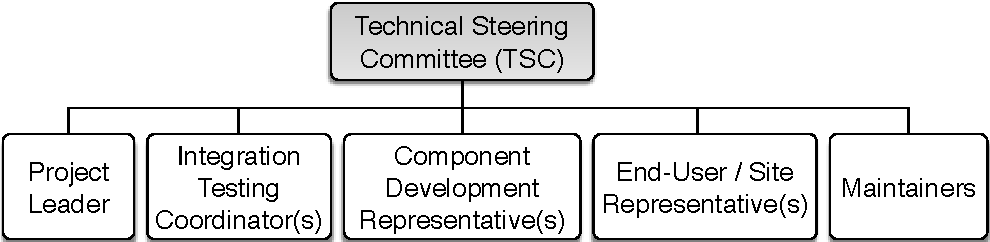
\includegraphics[width=1.0\linewidth]{figures/governance}
  \caption{Identified roles within the OpenHPC Technical Steering Committee (TSC).}
  \label{fig:tsc_governance}
\end{figure}

\subsection{Installation/Repository Overview}
\label{sec:repo_enable}

As mentioned previously, OpenHPC endeavors to adopt a repository-based delivery
model similar to the underlying OS distributions commonly used as the basis for HPC
Linux clusters.  At present, OpenHPC is providing builds targeted against two
supported OS distributions: CentOS7 and SLES12. The underlying package
managers for these two distributions are {\bf \texttt yum} and {\bf \texttt zypper},
respectively, and OpenHPC provides public repositories that are compatible with
these RPM-based package managers.

The installation procedure oulined in current OpenHPC recipes targets
bare-metal systems and assumes that one of the supported base operating systems
is first installed on a chosen {\em master} host. This is typically done
leveraging bootable media from ISO images provided by the base OS and once
installed, OpenHPC recipes highlight steps to install additional software and
perform configurations to use the {\em master} host to provision the remaining
cluster.

An overview of the physical infrastructure expected for use with
current OpenHPC recipes is shown in
Figure~\ref{fig:cluster_arch} and highlights the high-level networking
configuration. The {\em master} host requires at least two Ethernet interfaces
with {\em eth0} connected to the local data center network and {\em eth1} used
to provision and manage the cluster backend (note that these interface names
are examples and may be different depending on local settings and OS
conventions). Two logical IP interfaces are expected to each compute node: the
first is the standard Ethernet interface that will be used for provisioning and
resource management. The second is used to connect to each host's BMC and is
used for power management and remote console access. Physical connectivity for
these two logical IP networks is often accommodated via separate cabling and
switching infrastructure; however, an alternate configuration can also be
accommodated via the use of a shared NIC.
%, which runs a packet filter to divert
%management packets between the host and BMC.
For power management, we assume that the compute node baseboard management
controllers (BMCs) are available via IPMI from the chosen master host. For file
systems, the current recipe(s) document setting up the chosen master
host as an NFS file system that is made available to the compute
nodes. Installation information is also discussed to optionally include a
Lustre~\cite{Lustre_url} file system mount.

\begin{figure}[h]
  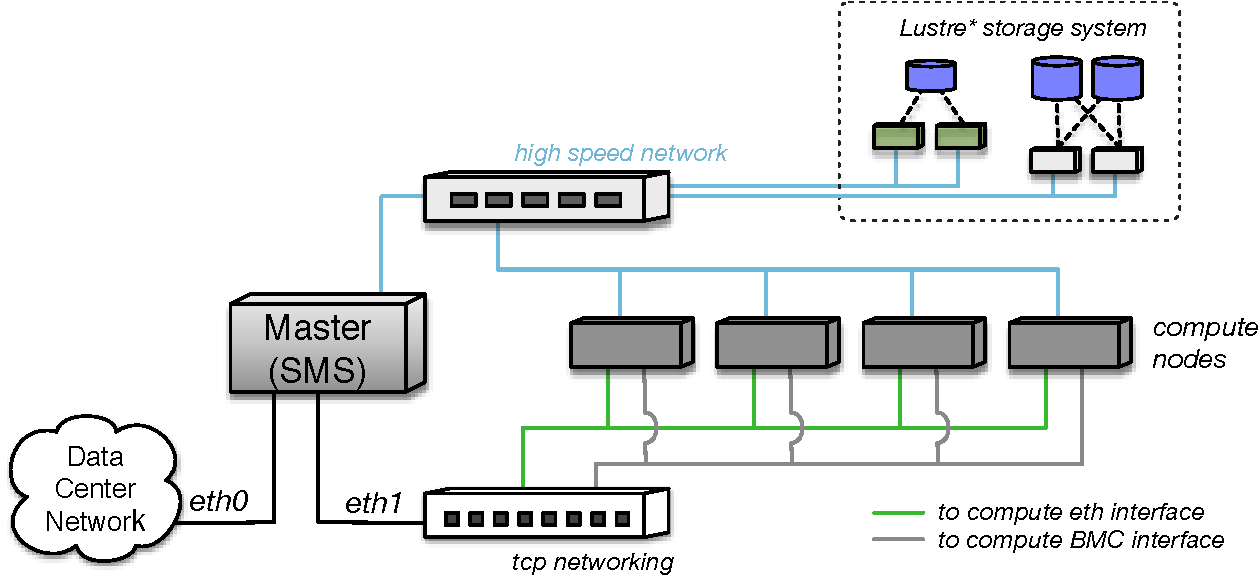
\includegraphics[width=0.95\linewidth]{figures/ohpc-arch-small.pdf}
  \caption{Overview of physical cluster infrastructure expected with OpenHPC
    installation recipes.}
  \label{fig:cluster_arch}
\end{figure}

\noindent{\bf Community Repo:} In cases where external network connectivity is
available on the {\em master} host, OpenHPC provides an \texttt{ohpc-release}
package that includes GPG keys for package signing and repository enablement.
This package can be downloaded from the OpenHPC GitHub community site directly
(\url{https://github.com/openhpc/ohpc}). Note that additional repositories may
be required to resolve package dependencies and, in the case of CentOS, access
to the EPEL~\cite{epel_url} repo is currently required.

The most recent release branch for OpenHPC is version~1.1 and the output in
Figure~\ref{fig:repolist} highlights the typical repository setup after
installation of the \texttt{openhpc-release-1.1} RPM in a CentOS
environment. Following typical OS distro conventions, note that two OpenHPC
repositories are enabled by default: a { \bf base} repo corresponding to the
original 1.1 release and an {\bf updates} repo that provides rolling fixes and
enhancements against the 1.1 tree.

\begin{figure}[h]
\begin{lstlisting}[language=bash,keywords={}]
(*\#*) yum repolist
repo id              repo name
OpenHPC              OpenHPC-1.1 - Base
OpenHPC-updates      OpenHPC-1.1 - Updates
base                 CentOS-7 - Base
epel                 Extra Packages for Enterprise...
\end{lstlisting}
\vspace*{-0.3cm}
  \caption{Typical package repository configuration after enabling OpenHPC
    (CentOS example).}
    \label{fig:repolist}
\end{figure}

%epel             Extra Packages for Enterprise Linux 7 - x86_64

\subsection{Packaging} \label{sec:packaging}

%Being building-block oriented in nature,
To highlight several aspects of the current packaging conventions, we next
present several installation examples. Note that this
discussion does not endeavor to replicate an entire install procedure, and
interested readers are invited to consult the latest installation recipe(s) that
are availble on the community GitHub site (or via the installable
\texttt{docs-ohpc} RPM) for more detailed instructions.

Once the OpenHPC repository is enabled locally, a range of packages are
available and a typical install on the {\em master} hosts begins with the
installation of desired system administration services. In the example that follows, the
Warewulf provisoning system is installed using available convenience groups:

\begin{lstlisting}[language=bash,keywords={}]
[sms](*\#*) yum -i groupinstall ohpc-warewulf
[sms](*\#*) yum -i groupinstall ohpc-slurm-server
\end{lstlisting}
  
Convenience groups like the examples above are prefixed with the ``ohpc-'' tag
and install a collection of related packages. As an example, the
\texttt{ohpc-warewulf} group expands to include all the packages needed to
enable a Warewulf provisioning server. Similarly, the
\texttt{ohpc-slurm-server} group includes the packages needed to stand up a
SLURM control daemon for resource management across the cluster.  Although not
shown here, a related \texttt{ohpc-slurm-client} group is also available to allow
for installation of a smaller set of packages needed to enable a SLURM client
(typically installed in compute node images).

Note that individual packages names provided via OpenHPC are appended with the
``ohpc'' suffix.
The motivation for this convention was to  allow for easy wild-carding queries with package managers, and
to also provide the ability to install OpenHPC-provided versions of software packages
along side alternate distro versions of the same packages (if available).
Finally, while the examples here continue to use the \texttt{yum} package
manager, equivalent commands can be substituted using \texttt{zypper} when
using SLES.  \\

\noindent {\bf Development Libraries}:
In addition to providing tools primarily targeted at system administrators, OpenHPC
also provides pre-packaged builds for a number of popular open-source tools and
libraries used by HPC applications and developers. For example, OpenHPC
provides builds for FFTW and HDF5 (including serial and parallel I/O
support), and the GNU Scientific Library (GSL). Again, multiple builds of
each package are available in the OpenHPC repository to support multiple
compiler and MPI family combinations where appropriate.
%Note, however, that not
%all combinatorial permutations may be available for components where there are
%known license incompatibilities.
The general naming convention for builds
provided by OpenHPC is to append the compiler and MPI family name that the
library was built against directly into the package name. For example,
libraries that do not require MPI as part of the build process adopt the
following RPM name: \\

\noindent
\texttt{package-<compiler\_family>-ohpc-<version>-<rel>.rpm} \\

\noindent Packages that do require MPI as part of the build expand upon this convention to
additionally include the MPI family name as follows: \\

\subsection{Conventions}
\subsubsection{Architecture}
%%We have assembled a variety of common ingredients required to deploy and manage 
%%an HPC Linux cluster including provisioning tools, resource management, I/O 
%%libraries, development tools, and a variety of scientific libraries. The 
%%delivery mechanism is via standard package managers (i.e., there are public 
%%OpenHPC repositories for both yum and zypper). OpenHPC currently supports CentOS
%%7 and SUSE's SLE 12. A single RPM spec file generates packages for both base
%%operating systems. This multiple target model also extends to compiler
%%toolchains and MPI runtime libraries. For some components that means a spec file
%%can generate 12 different versions of a package. This complexity is masked by
%%yum/zypper convenience groups, macros within the build system, and hierarchical 
%%Lmod environment modules for users.



--example showing convenience group installation, package name convention, module
load--

 - repo layout description

\subsubsection{Build}

 - spec file conventions
 - git + OBS
 
\subsubsection{Test}
 To facilitate global efforts in diagnostics/validation, we have devised a standalone integration test infrastructure
 • Intent was to create families of tests that could be used during:
 - initial install process (can we build a system?)
 - post-install process (does it work?)
 - developing tests that touch all of the major components (can we compile against 3rd party libraries, will they execute under resource manager, etc)
 • Expectation is that each new component included will need corresponding integration test collateral
 • These integration tests are included in GitHub repo


\section{Conclusions \& Future work}
Some known big ticket items on the horizon for the TSC
- establishing a process and prioritization/selection process for including
new software components
- establish minimum integration test expectations
- establish packaging conventions:
• naming schemes
• dependency hierarchy management • installation paths
• upgrade/rollback? mechanisms
- road map time line for next release (and cadence strategy for future releases)
- addition of public CI infrastructure, roll out of additional architecture builds

%ACKNOWLEDGMENTS are optional
%\section{Acknowledgments}

\bibliographystyle{abbrv}
\bibliography{hpcsyspros}


\end{document}
